\chapter[\texorpdfstring{Angular Distributions of the $^\text{12}$B\lowercase{($d$,$p$)} Measurement}{Angular Distributions of the 12B(d,p) Measurement}]{\texorpdfstring{Angular Distributions of the \newline $^\mathbf{12}$B($d$,$p$) Measurement}{Angular Distributions of the 12B(d,p) Measurement}}
\label{badang}
Following the discussion of \ref{b12_ang}, this chapter further details the method of analysis used for determining the angular distributions of $^{11}$B($d$,$p$) and $^{12}$B($d$,$p$).

The two states with the most statistics---the 2.62\,MeV and 3.39\,MeV excited states---were used to to calibrate the efficiency of the detector array.  The 3.39\,MeV excited state was populated with over 4$\times$ the statistics of any other state; this state was used to calibrate most of the array.  However, examination of Fig.~\ref{b11_spec} reveals that the 3.39\,MeV state (labeled d in the figure) does not extend onto detector position 1.  This position was calibrated with the 2.62\,MeV excited state (c in the figure).  Fig.~\ref{b12angdist2} illustrates the method of efficiency calibration. Following the procedure described in the previous chapter, the array is binned into equal ranges of $\Delta z$; in this case, each bin corresponds to half a detector detector.  The equal ranges of $\Delta z$ are equivalent to equal ranges of $\Delta \cos(\theta_\mathrm{cm})$, in this case $\Delta \cos(\theta_\mathrm{cm})=0.009$ or 2.3\,msr.  In the top panel of the figure, the un-normalized angular distribution is plotted with a DWBA calculation fitted to the points. 

In the lower panel in the figure, the data have been scaled by a ratio of DWBA/data.  Notice that all of the points in the 3.39\,MeV angular distribution, corresponding to detectors 2--6, lie on the DWBA calculation.  In addition, the first two points of the 2.62\,MeV angular distribution, corresponding to detector 1, also line up with the DWBA calculation. 

\begin{figure}%
\centering
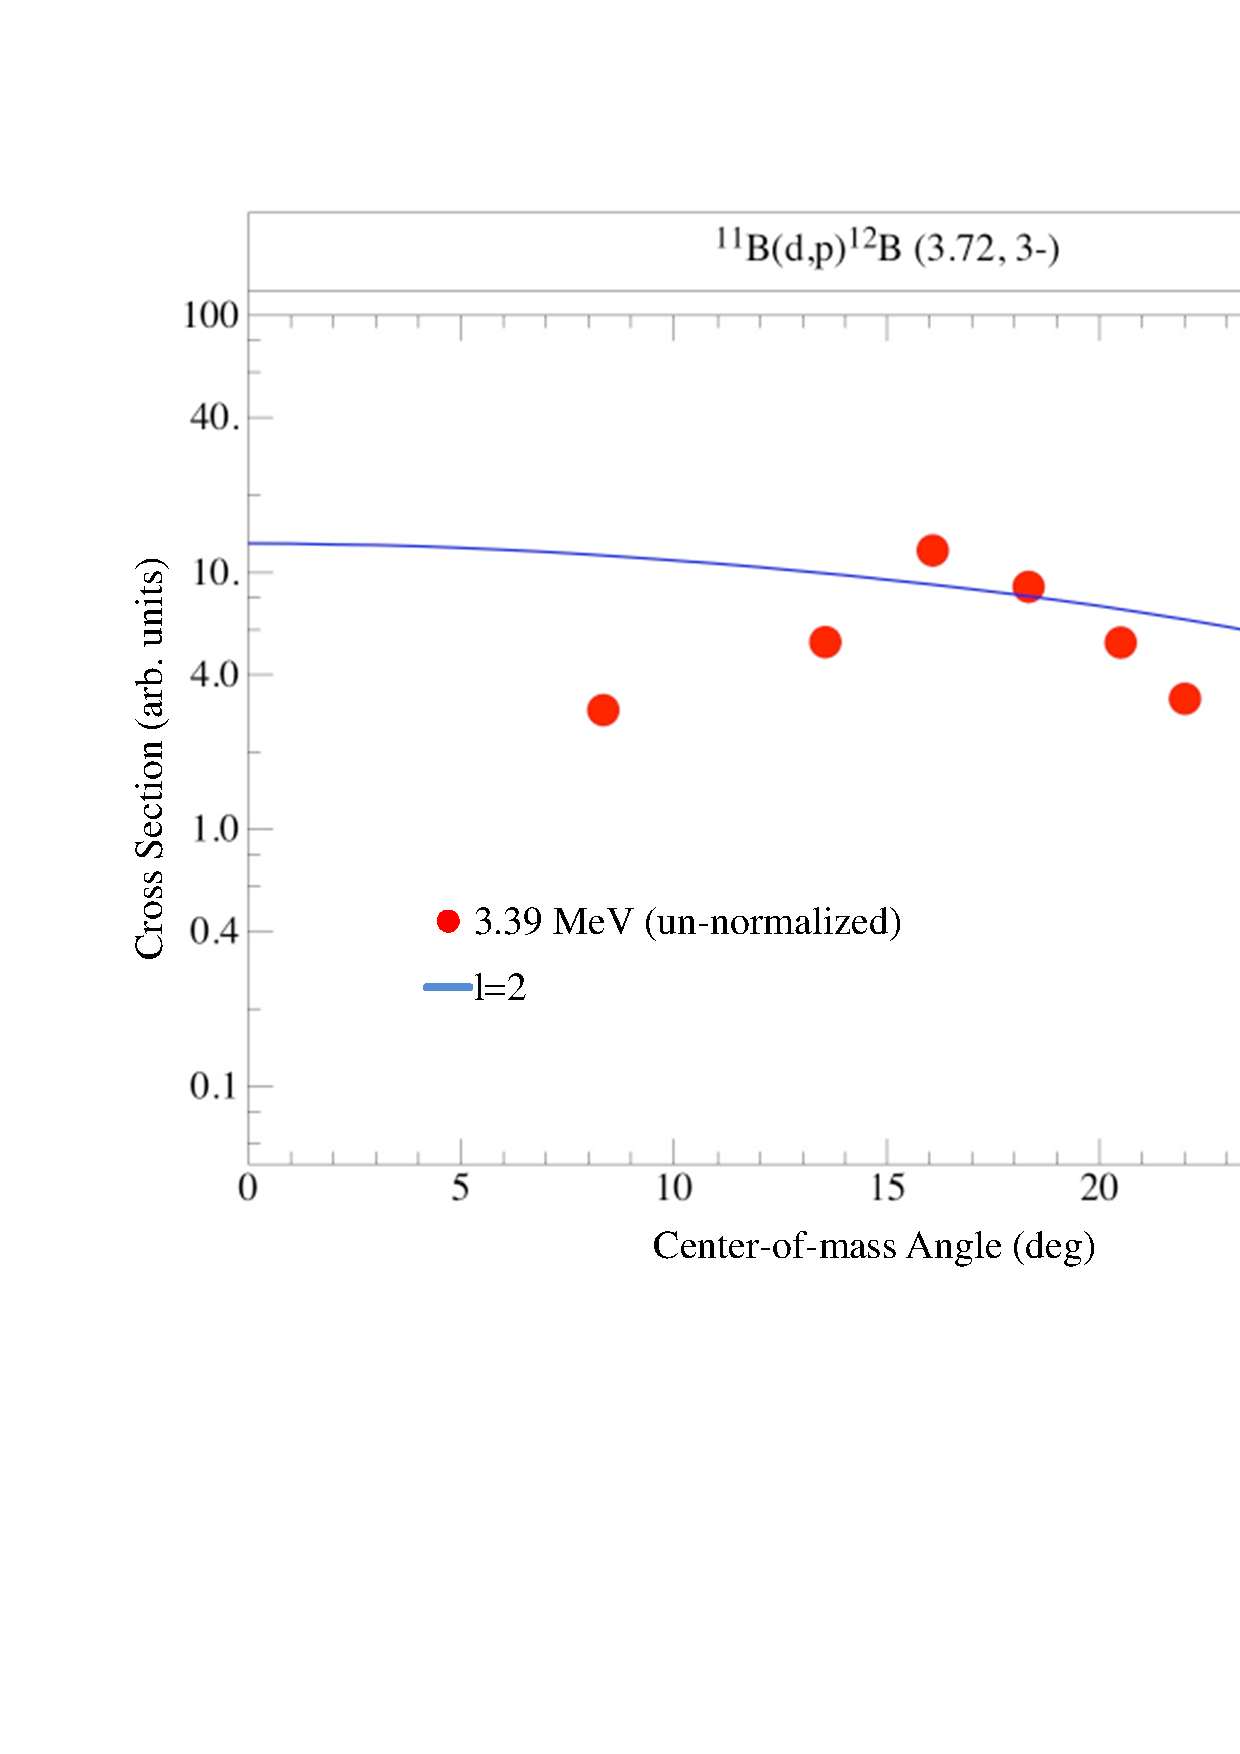
\includegraphics[height=0.45\textheight,width=\columnwidth,keepaspectratio]{More_Figures/b12_unnorm}\\
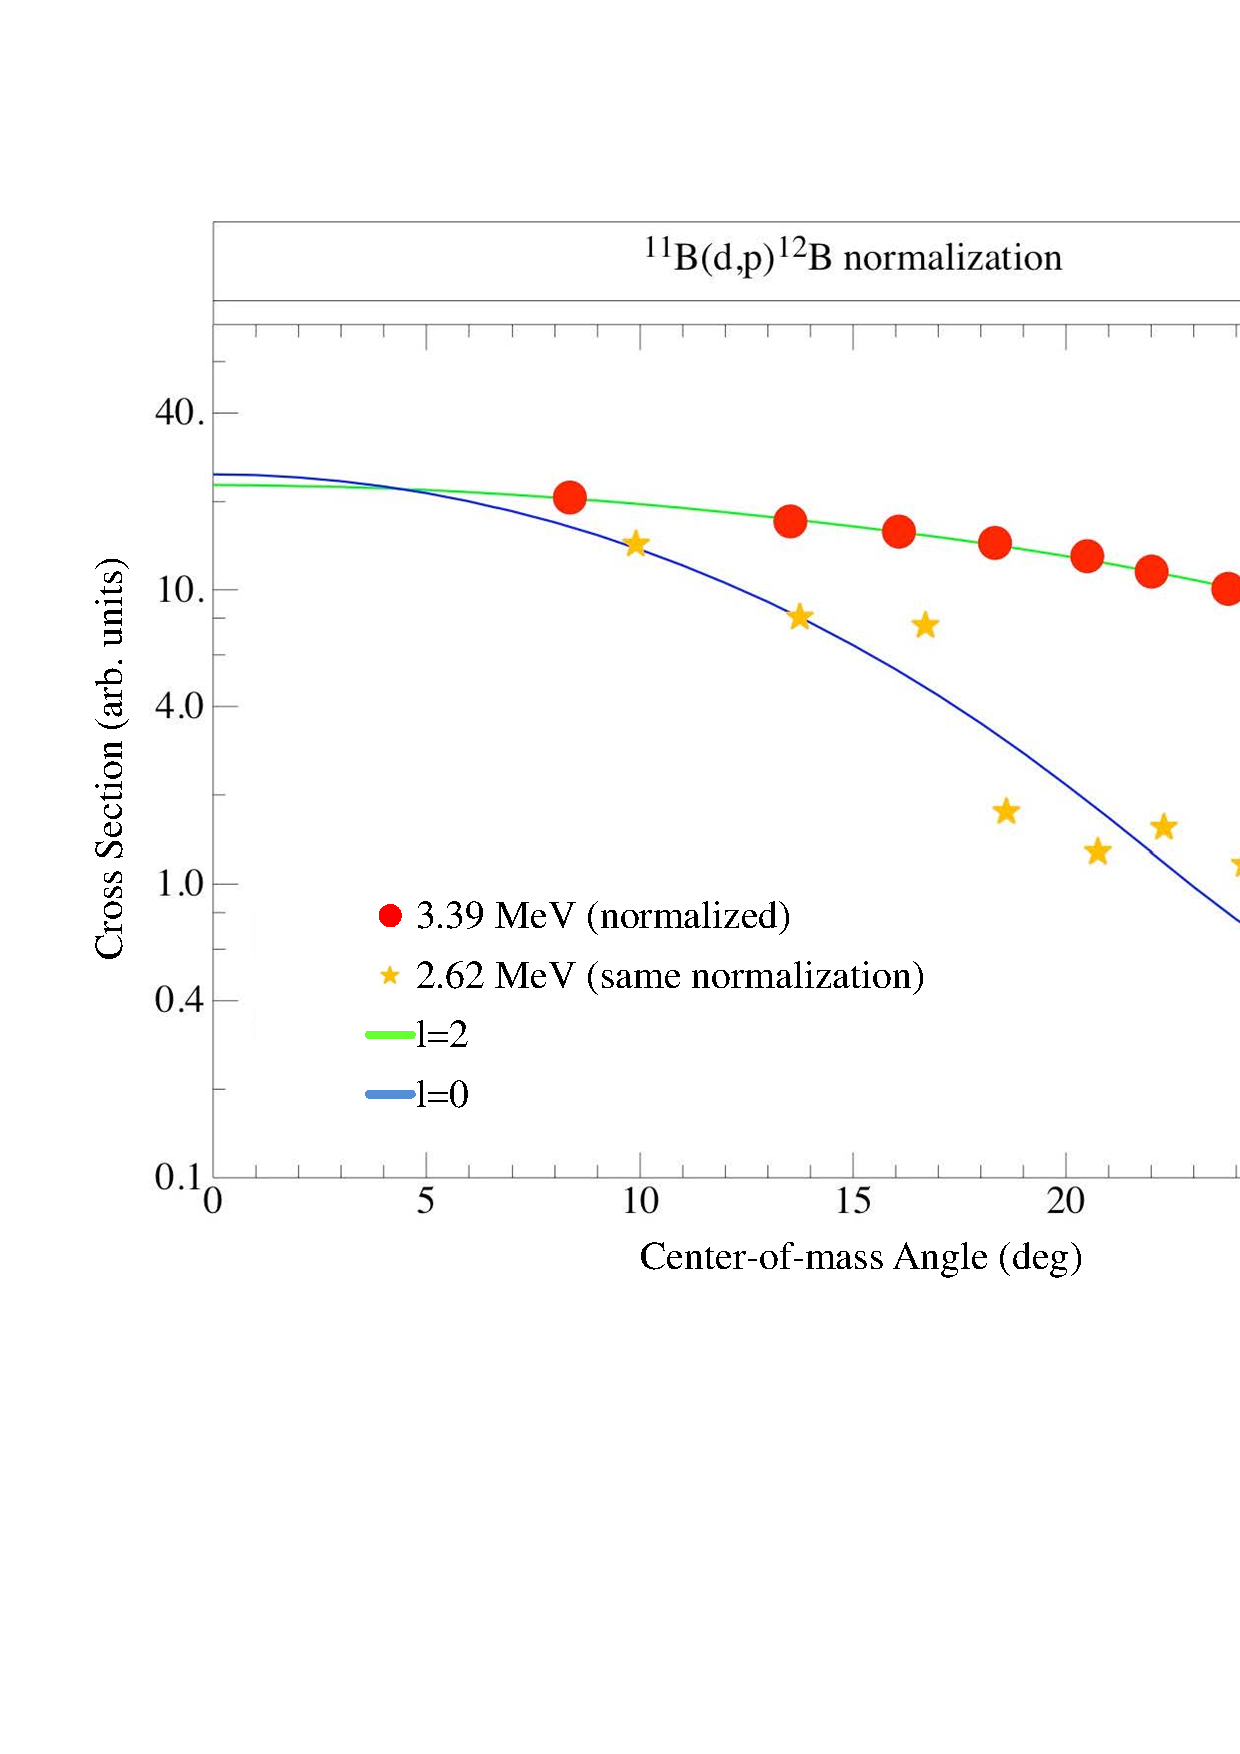
\includegraphics[height=0.45\textheight,width=0.98\columnwidth,keepaspectratio]{More_Figures/b12_norm}%
\caption[Illustration of the efficiency calibration technique]{Illustration of the efficiency calibration technique.  In the top panel the angular distribution of the 3.39\,MeV state ($\ell_n=2$) is fitted with a DWBA calculation.  In the bottom figure, the data points have been scaled by (DWBA/data), with each bin having the same efficiency correction. Figure annotated from Ref.~\cite{Schiffer_2009PC}.}%
\label{b12angdist2}%
\end{figure}

\begin{figure}[p]
\centering
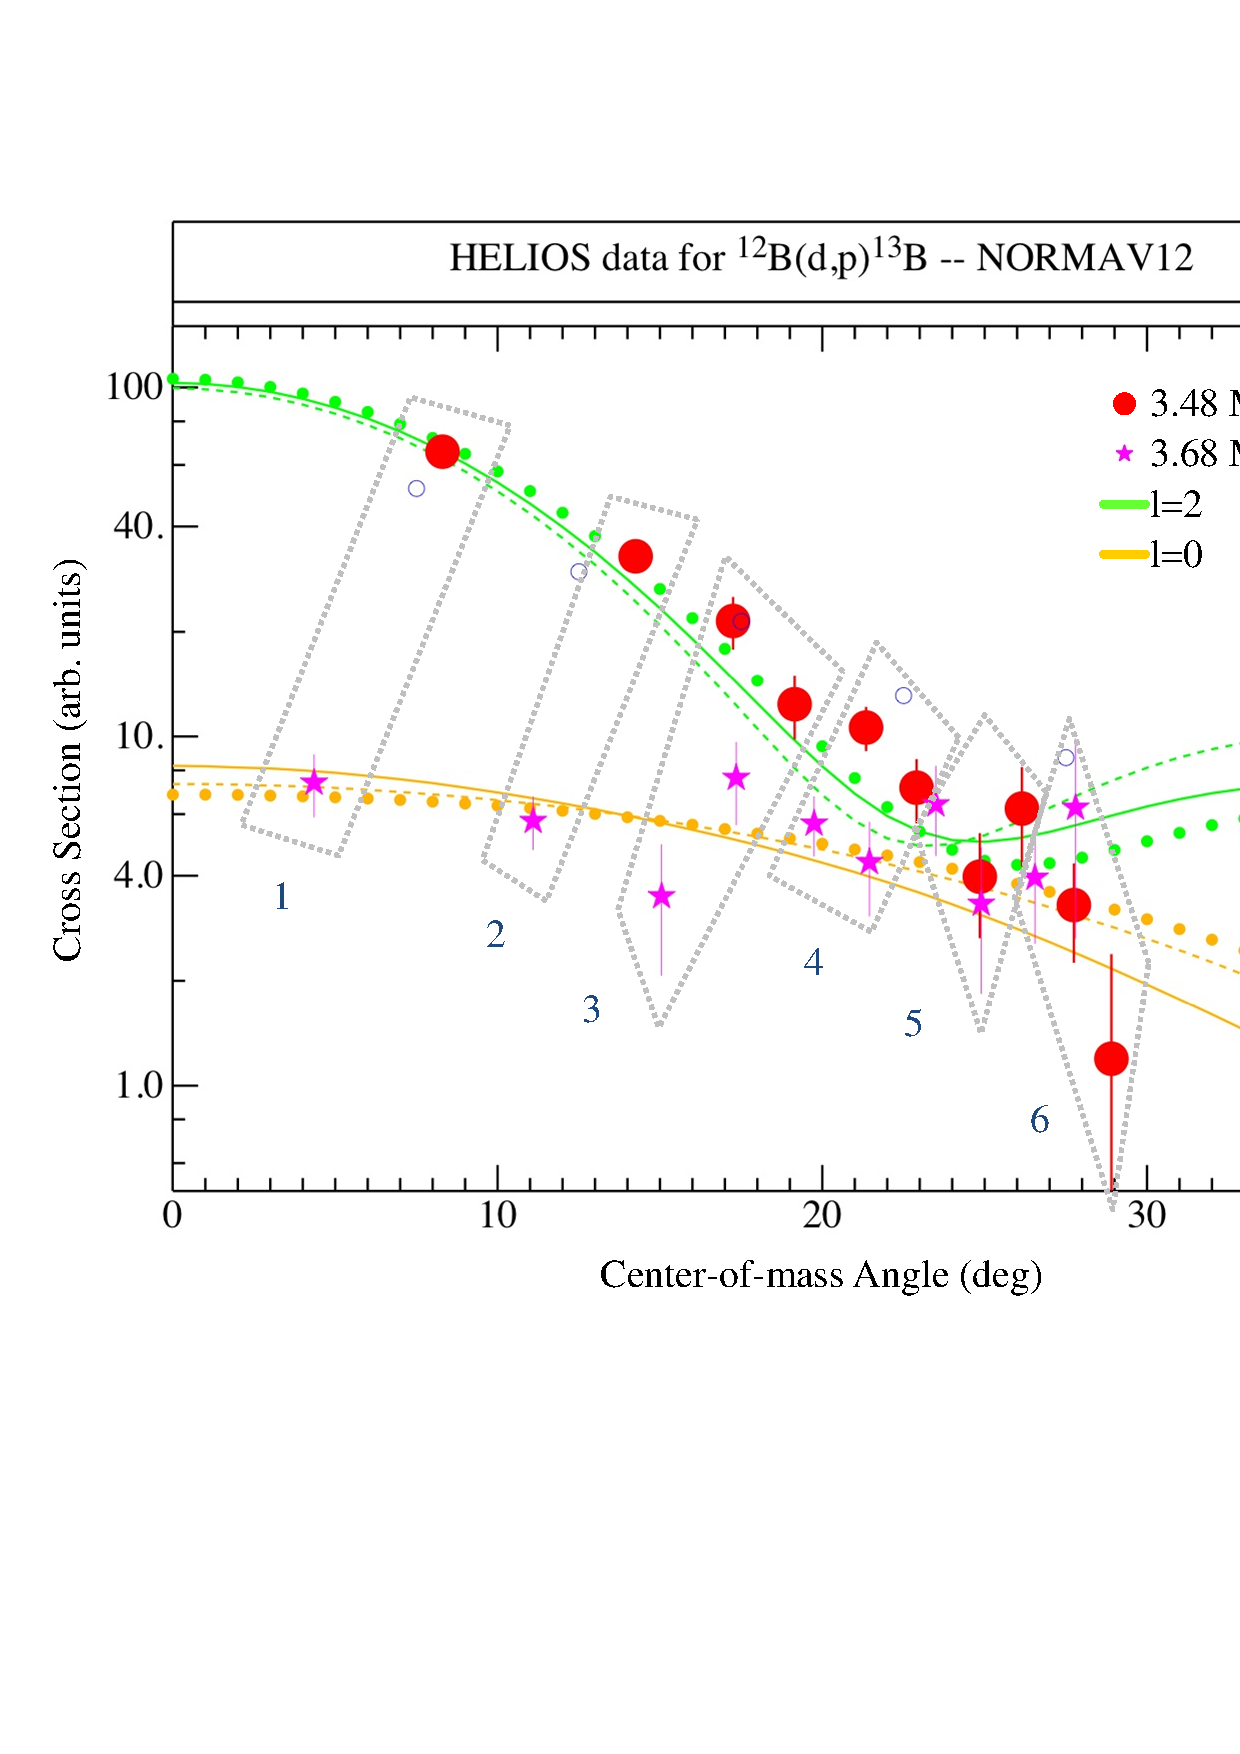
\includegraphics[height=0.4\textheight,width=\columnwidth,keepaspectratio]{More_Figures/b13}%
\caption[Angular distribution of of the $^{12}$B($d$,$p$) reaction]{Angular distribution of of the $^{12}$B($d$,$p$) reaction using the normalization derived from the $^{11}$B($d$,$p$) reaction.  DWBA calculations have been fit to the data using three different optical model parameters sets, discussed in Ref.~\cite{Schiffer_2010}. The quadrilateral boxes group data points corresponding to individual detector positions.  Please note that this is an annotated figure from a private communication~\cite{Schiffer_2009PC} and should be considered for illustrative purposes only.  The value of the angles plotted correspond to a target-to-detector separation of $\Delta z = 428$\,mm, which is consistent with using detector positions 1--5 only; however, as indicated in the figure, all six detector position are represented. This minor computational error is corrected in Ref.~\cite{Schiffer_2010}.
}%
\label{b13angdist}%
\end{figure}
